\begin{task}{72}
Из двух представленных ниже графов ровно один планарен. Перерисуйте планарный граф без пересечений рёбер, а в непланарном графе найдите подграф, гомеоморфный $K_{3,3}$.

\begin{center}
  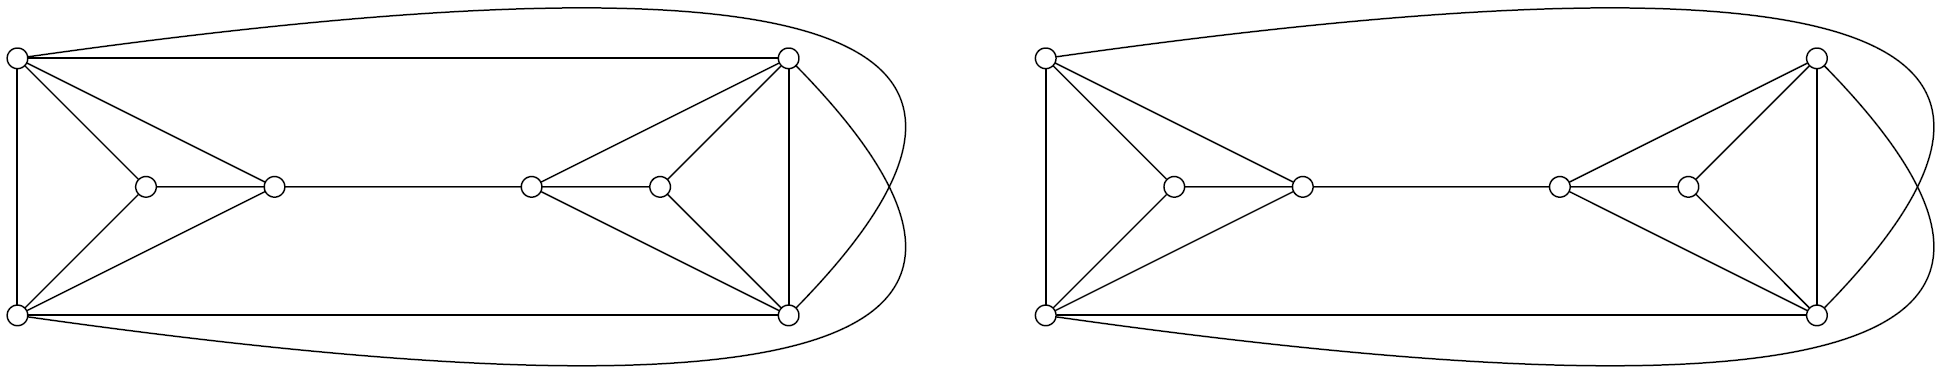
\includegraphics[width=0.8\linewidth]{72_1}
\end{center}
\end{task}

\begin{solution}
Выделим в первом графе $K_{3,3}$. По теореме Понтрягина — Куратовского он непланарный.
\begin{center}
  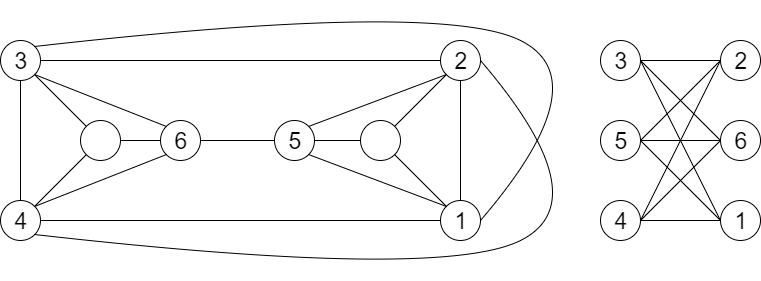
\includegraphics[width=0.8\linewidth]{72_2}
\end{center}
Перерисуем второй граф. Как видно, он планарный.
\begin{center}
  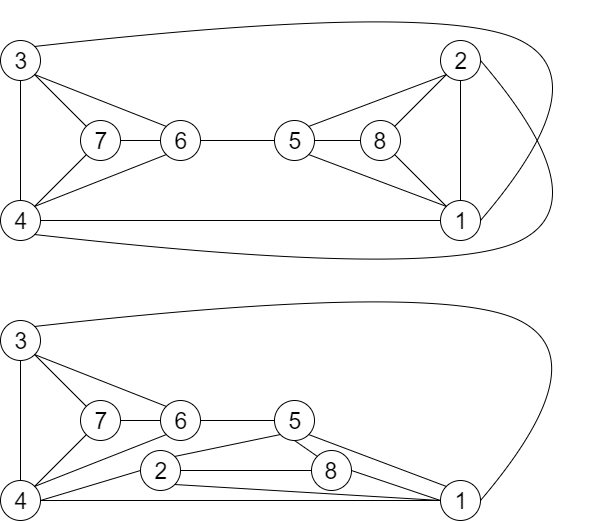
\includegraphics[width=0.6\linewidth]{72_3}
\end{center}
\end{solution}